\documentclass{article}
\usepackage{graphicx}
\graphicspath{ {./Pictures/} }
\usepackage[table,xcdraw]{xcolor}

\title{My Chapter}
\author
{Gabriela Czapska}
\date{31 October 2022}

\begin{document}

\maketitle
\tableofcontents

\section{Section0}
This is something created in Github and in VS Code that is to be read in Overleaf

\section{Introduction}
First, I'd like to say that my favourite physics equation is 
\[E=mc^2\]
And I'd \textbf{love} to \underline{go climbing} now

\begin{figure}[h!]
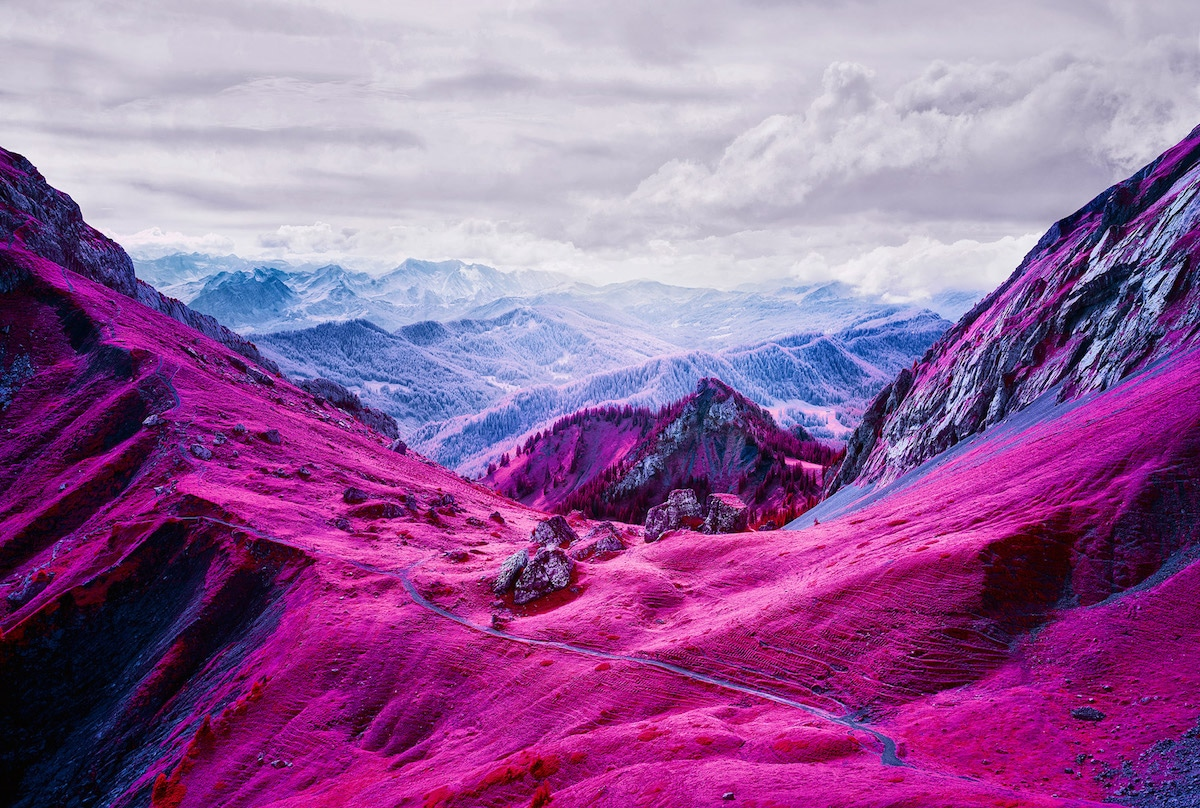
\includegraphics[width=\linewidth]{Pictures/mountains.jpg}
\caption{Pinky mountains}
  \label{fig:mountains}
\end{figure}


\begin{table}[]
\begin{tabular}{|l|l|l|l|l|}
\hline
\rowcolor[HTML]{DAE8FC} 
                          & A & B & C & D \\ \hline
\cellcolor[HTML]{DAE8FC}1 & X &   & X &   \\ \hline
\cellcolor[HTML]{DAE8FC}2 &   & X &   &   \\ \hline
\cellcolor[HTML]{DAE8FC}3 & X &   & X &   \\ \hline
\end{tabular}
\end{table}

\section{Another Part}
\centering

\begin{itemize}
  \item It is a first dot
  \item Here comes another
  \item And the other
\end{itemize}
\begin{enumerate}
  \item Number 1
  \item Number 2
  \item Number 3
\end{enumerate}
\end{document}
